\scanpage{43}
que pour tout segment $I$ de $S$, $I\subset S''$, il existe un plus grand segment de $S$ contenu dans $S'$ le contenant.

% slanted
\margin{introduire $\mathrm{Segm}_{\subset S'}(S\deleted{,\unsure{S'}})=\{I\subset S'\mid I\in\mathrm{Segm}(S)\}$}

Les éléments maximaux de $\mathrm{Segm}_{\subset S'}(S\deleted{,\unsure{S'}})$ sont appelés les \uline{segments \unsure{composants|comp.sants}} de la partie $S'$ de $S$.

% slanted
\margin{les \unsure{élém.} maximaux de $\mathrm{Segm}(S,S')$ i.e. les segments composants de $S'$, sont en corr. \unsure{1.1.} \unsure{resp.|pr.} \unsure{avec} les éléments \uline{minimaux} de l'ens des \deleted{\unsure{cl.|cl}} segments de $S$ qui \uline{contiennent} $S''$, par $I\mapsto S\setminus I$
\[
 \mathrm{Seg}_{\subset S'}(S)\overset{\unsure{\mathrm{antiiso.}}}{\simeq}\mathrm{Seg}_{\supset S''}(S)
\]}

Ils forment une partition de $S'$, d'où une relation d'équivalence dans $S'$.

En termes d'une réalisation top. de $(S,\{u,u^{-1}\})$ par un polygone top $(X,S)$, si $S''=S\setminus S'$, les \deleted{classes} segments de $S'$ sont en corr biunivoque avec les comp. conn. de $X\setminus S''$ qui rencontrent $S'$ -- ce sont les intersections de $S'$ avec ces comp. connexes.
\figure{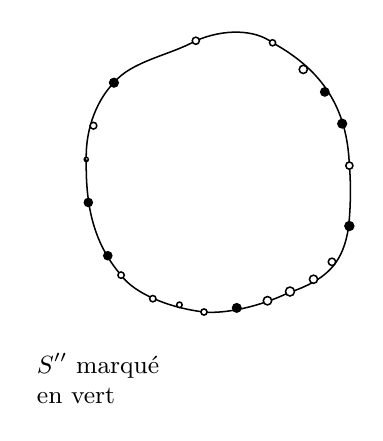
\begin{tikzpicture}[x=.013cm,y=-.013cm,line width=.55pt]
\draw (139,1183) .. controls (156,1162) and (194,1156) .. (219,1142)
 .. controls (247,1130) and (277,1131) .. (294,1144)
 .. controls (343,1171) and (367,1208) .. (369,1264)
 .. controls (371,1285) and (370,1316) .. (367,1331)
 .. controls (361,1360) and (346,1376) .. (310,1388)
 .. controls (281,1402) and (247,1409) .. (227,1407)
 .. controls (193,1403) and (159,1389) .. (146,1371)
 .. controls (121,1342) and (111,1307) .. (112,1258)
 .. controls (111,1226) and (124,1198) .. (139,1183) -- cycle;
\foreach \x/\y/\r in {219/1142/3.5,294/1144/3,324/1170/4,369/1264/3.5,352/1358/3.6,334/1375/4,311/1387/4.4,289/1396/4.1,227/1407/3,203/1400/2.7,177/1394/3.1,146/1371/3.1,119/1225/3.3}
  \draw[fill=white] (\x,\y) circle[radius=\r];
\foreach \x/\y/\r in {139/1183/5,345/1192/4.8,362/1223/5,369/1323/5.1,259/1403/4.9,133/1352/4.7,114/1300/4.7,112/1258/2.8}
  \fill (\x,\y) circle[radius=\r];
\fill[white] (112.5,1257.5) circle[radius=.8];
\node[anchor=west,align=left,font=\small] at (54,1472) {$S''$ marqué\\en vert};
\end{tikzpicture}}

\uline{Proposition} Soient $A,B$ deux parties \deleted{disjointes non vides} de $S$, on suppose \deleted{$A$ et $B$}
\[
 A,B\ne\varnothing,S,\qquad A\cap B=\varnothing.
\]

Conditions équivalentes

% slanted
\margin{\uline{NB} On peut \inserted{\unsure{prendre}} pour $\bar A,\bar B$ les \inserted{\unsure{plus|des}} \deleted{\unsure{petits}} \deleted{\unsure{segments|sgmts}} \unsure{composants|correspondants}}

a) $\exists$ segments $\bar A,\bar B$ de $S$, tels que $\bar A\supset A,\bar B\supset B$, $\bar A\cap\bar B=\varnothing$
% archive sheet number: 42
